\chapter{Algoritmo Genético}

\section{Introducción}
%
Se seleccionó un algoritmo genético para realizar la optimización de la
geometría del MRCVC por la simplicidad y facilidad de implementación.
%
Si bien estos métodos no garantizan que se alcance un resultado óptimo, en la
práctica\cite{goldberg}\cite{shi} se ha observado que alcanzan soluciones muy
cercanas a las óptimas tras pocas iteraciones del método.
%
Una de las ventajas de este método es que no requiere información del gradiente
de la función que se está evaluando, lo cual es útil cuando no se puede
asegurar la existencia de la derivada de la función en todo el dominio ó cuando
se tiene una función con más de un máximo o mínimo local.
%
Además, el punto de partida de la optimización es una población generada al
azar, de modo que se tiene un muestreo aleatorio del dominio que se está
evaluando.
%
Esto hace que el método sea poco susceptible a caer en un óptimo local.

Se puede decir que un algoritmo genético es un método de búsqueda aleatoria
guiada.
%

Gran parte de este trabajo fue fue utilizar a ICESym como parte de la función
con la que se evalúan los motores.
%
Para lograr esto se modificó parte del código de ICESym, con el objetivo de
facilitar la lectura de los resultados que arroja el simulador.
%
Además, se es necesario poder ejecutar de manera automatica una simulación con
una configuración particular del motor.
%
Otro aspecto del optimizador que se desarrolló es el de poder ejecutar
múltiples instancias de ICESym en paralelo, para poder aprovechar el hecho de
que los CPU's modernos tiene más de un núcleo físico, pudiendo ejecutar
múltiples procesos de manera simultánea y así reducir el tiempo de ejecución de
las simulaciones. 
%

\subsection{$r_v = ICESym(motor)$}
%
ICESym lee un archivo de configuración en formato \emph{Python} que consta de
un arrego llamado \emph{diccionario} con las siguientes entradas

\begin{lstlisting}[language=Python]
kargs = {
    "Simulator": Simulator,
    "Cylinders": Cylinders,
    "Junctions": Junctions,
    "Tubes": Tubes,
    "Tanks": Tanks,
    "Atmospheres": Atmospheres,
}
\end{lstlisting}

En donde se guarda la información básica de la geometría del motor, modelos
termodinámicos utilizados, cantidad de RPM's a simuilar y modelo de Cd entre
otros.

% De manera resumda, son básicamente métodos de búsqueda aleatoria que
% aprovechan la información de iteraciones previas para determinar la composición
% futura de la población, representando individuos como un conjunto de datos.
% La representación
% %
% Si bien es probable que no se alcance el óptimo, el método alcanza una solución
% satisfactoria en un tiempo relativamente corto.

¿Cómo difieren los AG de los métodos tradicionales de búsqueda?
%
\begin{enumerate}
    %
  \item Los AG trabajan sobre una representación de las variables estudiadas y
      no necesariamente sobre las variables de estudio.
        % Por ejemplo una una representación binaria de conjunto de decimales.
    %
    \item Trabajan con un conjunto de datos, no con un solo punto.
    %
    \item Utilizan una función objetivo para evaluar cada punto de datos, sin
        necesidad de conocer la derivada de la función que se está evaluando.
    %
    \item Los AG usan reglas probabilísticas, no deterministas.
    %
\end{enumerate}

% Los AG requieren que las variables del problema estén expresadas en forma de
% coordenadas $(x_1, x_2, x_3, ..., x_n)$.

Otros métodos de optimización se mueven de un punto al siguiente en el espacio
solución, basándose en alguna regla de decisión, esto puede ser riesgo porque
se puede caer en un óptimo local.

El proceso de optimización se puede resumir en:

Crear una población al azar
generación actual < total generaciones do
evaluar la población
Seleccionar los individuos que formarán la próxima generación
Cruzar los candidatos seleccioados y crear la nueva población
Mutar a los individuos de la nueva población


\section{Componentes básicos}
%
Un AG se puede construir con 3 operadores básicos:
\begin{enumerate}
    \item Reproducción
    \item Cruza
    \item Mutación
\end{enumerate}

La reproducción consiste en crear individuos a partir del puntaje que devuelve
en la función objetivo, la función objetivo es una medida del valor que
queremos optimizar.
%
Este paso significa que aquellos individuos que tengan valores, por ejemplo más
altos, de función objetivo tendrán más posibilidades de ser "copiados", de esta
forma se imita a la selección natural.

La cruza consiste en combinar los "vectores" de dos individuos para obtener uno
nuevo.

La mutación consiste en modificar aleatoriamente uno o más parámetros de cada
nuevo individuo.

Estos 3 simples mecanismos le dan a los AG su ¿poder?

La mutación juega un rol secundario pero muy importante, es secundario porque
se pueden alcanzar soluciones satisfactorias sin incluir este mecanismo, sin
embargo se utiliza con probabilidades pequeñas para evitar la pérdida temprana
de información relevante.
%
Si la probabilidad de mutación es muy alta, el AG se convierte en una simple
búsqueda aleatoria.

\section{\emph{Schema} y paralelismo implícito}

\emph{Schema} o esquema es una plantilla, un subconjunto de los parámetros que
definen al individuo en un AG que contienen información relevante al problema
en estudio.
%
Estas plantillas surgen de similitudes en posiciones y valores que dan buena
aptitud a un individuo.
%
Un AG procesa $n$ individuos y $n^k$ \emph{schematas} por iteración
\cite{goldberg}, cuanto mayor sea el tamaño del \emph{schema}, mayor la
probabilidad de ser truncado durante la cruza o mutación, esto produce que los
patrones de menor tamaño tengan mayor probabilidad de supervivencia de una
generación a otra.
%
Este proceso en el que bloques de información de menor tamaño al total de
parámetros que se está evaluado sobreviven de una generación a otra sin
necesidad de ingresar alguna modificación algoritmo es conocido como paralelismo
implícito.

\section{Implementación}
%
Para la primer iteración se programaron los algoritmos y funciones necesarias
para llevar a cabo la optimización desde cero.
%
Posteriormente se tomo la la librería DEAP \cite{DEAP_JMLR2012} y se
modificaron los operadores a medida, para poder utilizarlos con ICESym.

\subsection{Población}
%
Los parámetros que representan a cada individuo son los que definen la geometría
del sistema de intercambio de gases, estos son:

\begin{enumerate}
    \item [DTA] Diámetro de tubo de admisión.
    \item [DTE] Diámetro de tubo de escape.
    \item [LIT] Largo de tubo de admisión.
    \item [LET] Largo de tubo de escape.
    \item [IIA] Ángulo geométrico de apertura de puerto de admisión.
    \item [IFA] Ángulo geométrico de cierre de puerto de admisión.
    \item [IIE] Ángulo geométrico de apertura de puerto de escape.
    \item [IFE] Ángulo geométrico de cierre de puerto de escape.
\end{enumerate}

Los diámetros pueden tomar valores de hasta 100mm, el largo de los tubos puede
variar entre 500 y 1000 mm.
%
Con respecto al par de ángulos que marcan la apertura y cierre del ecape,
el único requisito es que la apertura se de antes que el escape.

\begin{lstlisting}[language=Python]
def check_angles(eng):
    """ Validates intake/exhaust angle pair"""
    iia = eng[-4]
    ifa = eng[-3]
    eia = eng[-2]
    efa = eng[-1]
    valid = True
    if iia >= ifa:
        valid = False
    if eia <= efa:
        valid = False
    return valid
\end{lstlisting}

Cada una de las variables se representa como un número binario de 5 dígitos,
los cuales se concatenan para formar un conjunto de 40 dígitos.
%

\begin{table}
    \centering
        \begin{tabular}{rc} \toprule
            0011001110110010001100110010011010100110 $ () \toprule
            1101011100001100010110011000001110110100 $ () \\ \midrule
            1101110101001010110000011000010110101010 $ () \\
            0010010111111010100101111111010011010001 $ () \\
            0100101110101111110110011001101011011100 $ () \\ \bottom
        \end{tabular}
    \caption{Binario a numeros}
    \label{tab:mapeo}
\end{table}

El orden de los mismos se mantiene constante, por lo que cada sección del número
representa una característica en particular del motor, de modo que:

\begin{equation}
    INDIVIDUO = (DTA, DTE, LIT, LET, IIA, IFA, EIA, EFA) \nonumber
\end{equation}

Este número luego se convierte a decimales y se mapea a la lista que se utiliza
para generar el archivo de configuración para ICESym.
%

\begin{lstlisting}[language=Python]
def map_to_engine(num, bin_len):
    t = utils.separate_list(num, bin_len)
    dta = (d_coeff[0]*utils.bin2dec(t[0]) + d_coeff[1]) * 0.001
    dte = (d_coeff[0]*utils.bin2dec(t[1]) + d_coeff[1]) * 0.001
    lit = (l_coeff[0]*utils.bin2dec(t[2]) + l_coeff[1]) * 0.001
    let = (l_coeff[0]*utils.bin2dec(t[3]) + l_coeff[1]) * 0.001

    iia = a_coeff[0]*utils.bin2dec(t[4]) + a_coeff[1]
    ifa = a_coeff[0]*utils.bin2dec(t[5]) + a_coeff[1]
    eia = a_coeff[0]*utils.bin2dec(t[6]) + a_coeff[1]
    efa = a_coeff[0]*utils.bin2dec(t[7]) + a_coeff[1]
    ind = (dta, dte, lit, let, iia, ifa, eia, efa)
    return ind
\end{lstlisting}

El tamaño de la población se elige arbitrariamente en $N=100$ individuos, 

\subsection{Reproducción}

Para crear la nueva población se debe elegir a los nuevos candidatos basándose
en los puntajes de la población actual, por medio de un método de selección de
tipo torneo, (iba por aca)
%


\subsection{Cruza}
%
El operador de cruza se encarga de combinar los genes de dos individuos para
producir un individuo nuevo.

El operador seleccionado es el de curza de dos puntos, en el que se seleccionan
al azar dos índices


\subsection{Mutación}
%
La mutación juega un rol secundario pero importante, una pequeña probabilidad
de que alguno de los genes se modifique en un valor aleatorio contribuye a que
el algoritmo genético no se estanque en soluciones máximos o mínimos locales.

\subsection{Función objetivo}
%
La función objetivo es la encargada de dar puntaje a los individuos, en la
analogía con la selección natura, esta función es el ambiente, el que determina
que tan bien se desempeña un motor con respecto a otro en lo que respecta a
rendimiento volumétrico.
%
Inicialmente se propuso que la función objetivo sea la suma de los rendimientos
volumétricos a todas las velocidades simuladas, este tipo de funciones da como
resultado una curva de rendimiento volumétrico aserrada como se muestra en la
figura (falta).

Este comportamiento aserrado es poco deseable, por lo que se modificó la
función para conseguir una curva de rendimiento volumétrico suave.
%
Además se implementó una suma ponderada, para obtener un rendimiento
volumétrico máximo en un valor arbitrario de 5000 RPM.

Para prevenir el comportamiento aserrado se introdujo un sistema de
penalidades, que resta puntaje si la derivada de la función se modifica de una
velocidad a otra.


Otro tema a tener en cuenta es la convergencia prematura del algoritmo que es
causado por es la dominancia temprana de unos pocos individuos con puntaje
superior al resto de la población.
%
Para evitar esto se realiza un cambio de escala puntaje de todos los
individuos, alguno de los métodos utilizados son: transformación lineal,
truncado $\sigma$ y transformación exponencial.
%
El método seleccionado es la transformación lineal, que funciona bien
\cite{goldberg} si no se tienen valores de aptitud negativos.

\begin{equation}
    f' = af + b
\end{equation}

Los coeficientes $a$ y $b$ se eligen de modo tal de que haya unicidad entre el
puntaje sin modificar y el transformado, otra función es que se asigne un
puntaje de 2 a los individuos con mayor puntaje, lo que asegura que para
puntajes medios tengan posibilidades de generar un individuo como descendencia y
los mejores individuos tengan múltiples "hijos".

\section{Implementación}


\subsection{Representación de los individuos}

Para representar a cada individuo se utilizan 8 características geométricas:

\begin{enumerate}
    \item [DTA] Diámetro de tubo de admisión.
    \item [DTE] Diámetro de tubo de escape.
    \item [LIT] Largo de tubo de admisión.
    \item [LET] Largo de tubo de escape.
    \item [IIA] Ángulo geométrico de apertura de puerto de admisión.
    \item [IFA] Ángulo geométrico de cierre de puerto de admisión.
    \item [IIE] Ángulo geométrico de apertura de puerto de escape.
    \item [IFE] Ángulo geométrico de cierre de puerto de escape.
\end{enumerate}


% NOTA: antes de esto tendría que explicar como funciona icesym y como
interactúa mi programa.  Con esta lista de decimales luego se generan los
archivos de alzada que representan la apertura de la válvula, la misma es una
alzada ficticia que se utiliza para calcular el área de referencia de puerto.

\begin{equation}
  A_{C} = \pi \cdot D_{v}\cdot l_{v}
\end{equation}

El área de referencia utilizada por ICESym es el área de cortina, esquematizada
en la figura \ref{fig:area_cortina}.

\begin{figure}
  \centering
  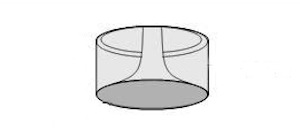
\includegraphics[width=0.5\textwidth]{valve_curtain.jpg}
  \caption{Área de cortina}
  \label{fig:area_cortina}
\end{figure}

Con la población definida se procede a los evaluar cada motor con la función
objetivo, la cual se definió de manera tal de favorecer curvas de rendimiento
volumétrico suaves y valores altos a mayores RPM.

La suavidad de la curva de rendimiento volumétrico se calcula midiendo los
cambios de pendiente de la derivada la cual se aproxima con la fórmula de
diferencia progresiva \ref{eq:derivada}.
%
Solamente interesa el signo, por lo que el valor de $h$ en el denominador no
interesa y se hace 1, con esto la función objetivo queda como el algoritmo
\ref{alg:funcObj}.

\begin{equation}
  f' = \frac{f(i+1) - u(i)}{h}
  \label{eq:derivada}
\end{equation}

\begin{lstlisting}[language=Python]
def evaluate_engine(individual, binnary_len, eng_obj, cores):
    """Takes a global instance of motor.MRCVC and calculates it's score based on
    volumetric efficiency curve.
    """
    if binnary_len:
        eng = map_to_engine(individual, binnary_len)
    else:
        eng = individual
        print(eng)
    if m.check_angles(eng):
        config = m.list_to_config(eng)
        counter = 0
        run_flag = False
        while counter < 2:
            print("counter", counter)
            kargs, cyl_data, extras_data = m.run_and_read(eng_obj, config, multi=cores)
            # kargs, cyl_data, extras_data = m.read(ENGINE_OBJ, config)
            vol_eff = m.calc_volumetric_efficiency(kargs, extras_data)
            print("vol eff", vol_eff)
            if 0 in vol_eff:
                counter += 1
            else:
                run_flag = True
                break
        if run_flag is False:
            return False
    else:
        return False
    return vol_eff
\end{lstlisting}

El conjunto de pesos utilizados para ponderar los rendimientos es el indicado
en la tabla \ref{tab:pesos}

\begin{table}
  \centering
  \begin{tabular}{rccccccccc} \toprule
      RPM  & $w$ \\ \midrule
      1000 & 1 \\
      2000 & 1 \\
      3000 & 1 \\
      4000 & 6 \\
      5000 & 8 \\
      6000 & 9 \\
      7000 & 8 \\
      8000 & 7 \\
      9000 & 7 \\ \bottomrule
  \end{tabular}
  \caption{Pesos}
  \label{tab:pesos}
\end{table}


Una vez evaluados todos los motores de la población, se debe seleccionar los
individuos que forman la población para la siguiente iteración.
%
El método de selección es de tipo TORNEO, en el cual se seleccionan los mejores
$k$ individuos de un grupo al azar de $N$ candidatos.
%

Con los nuevos candidatos seleccionados, se procede a variar la población,
realizando la cruza y mutación.

Luego se toman pares de individuos y de acuerdo a la probabilidad de cruza, se
combinan con el método seleccionado.

Finalmente se realiza una segunda iteración sobre la nueva población, aplicando
el método de mutación a cada individuo, de acuerdo a la probabilidad de
mutación indicada.


El método de cruza seleccionado es \emph{cruza de dos puntos}, en este método
se corta el vector que forma al individuo en dos puntos, la posición de estos
puntos se selecciona al azar, manteniendo el largo original de los vectores.
%
Luego los individuos ``cruzados'' se combinan de forma complementaria, como en
la figura \ref{fig:cr2puntos}

\begin{figure}
  \centering
  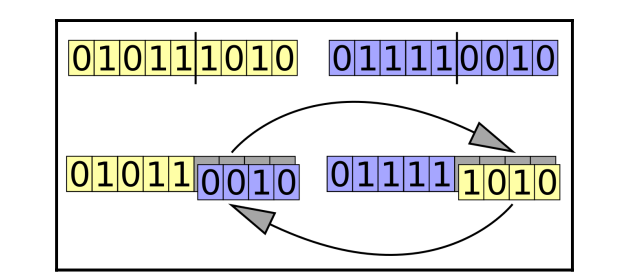
\includegraphics[width=0.5\textwidth]{cruza2puntos.png}
  \caption{Cruza de dos puntos}
  \label{fig:cr2puntos}
\end{figure}

% \begin{algorithm}
% \caption{Cruza de dos punos}\label{alg:c2puntos}
% \begin{algorithmic}[1]
% \Procedure{Cruza}{$a,b,n$}
%
%   \State $i\gets random(1:n)$
%   \State $j\gets random(1:n)$
%
%   % Aprox de la derivada
%   \For{$i=1:N$}
%     \State $d[i]\gets r[i+1]-r[i]$
%   \EndFor
%
%   % Calculo de la penalidad
%   \For{$i=1:N-1$}
%     \If{$d[i] \cdot d[i+1] < 0$}
%       \State $p\gets p + 1$
%     \EndIf
%   \EndFor
%   \State $p \gets 1 - \frac{p}{N-1}$
%
%   % Puntaje bruto
%   \State $w \gets 0$\Comment{Puntaje sin penalizar}
%   \For{$i=1:N$}
%     \State $w \gets r[i] \cdot w[i]$
%   \EndFor
%
%   % Puntaje con penalidad
%   \State $s \gets w \cdot p$
%   \State \textbf{return} $s$\Comment{s es el puntaje de la curva de rendimiento
%     volumétrico}
%   \EndProcedure
% \end{algorithmic}
% \end{algorithm}

El método de mutación seleccioand es mutShuffleIndexes (también podria se
mutFlipBit), en el cual se modifica el orden los números que componen al vector,
dando lugar a por ejemplo:

(figura con ejemplo)
